%---------------------
% START OF PREAMBLE - do not delete!
%---------------------
\documentclass[12pt]{article}
\usepackage[pdftex]{graphicx}
\usepackage{amsmath}
\usepackage{verbatim}
\usepackage{float}
\DeclareGraphicsRule{*}{mps}{*}{}

%==============================================================================
% Page layout
%==============================================================================

%------------------------------------------------------------------------------
%  Define the page dimensions.
%------------------------------------------------------------------------------
\setlength{\hoffset}{0.0in}
\setlength{\oddsidemargin}{0.0in}
\setlength{\evensidemargin}{0.0in}
\setlength{\textwidth}{6.75in}

\setlength{\voffset}{0in}
\setlength{\topmargin}{-.6in}
\setlength{\headheight}{12pt}
\setlength{\headsep}{12pt}
\setlength{\textheight}{9.5in}
\renewcommand{\baselinestretch}{1.0}
\renewcommand{\labelitemi}{-}

% writing the section number and the subsection number together
% and also the subsubsection in the form of 1.a
\renewcommand\thesubsection{\arabic{section}.\alph{subsection}}
\renewcommand\thesection{Problem \arabic{section}}
%------------------------------------------------------------------------------

%---------------------
% END OF PREAMBLE - do not delete!
%---------------------
\begin{document}

%---------------------
% make the title
%---------------------
\begin{titlepage}
\centering
{\LARGE\bfseries Homework 3}

\vspace{1cm}

{\Large Aerosol Physics, Chemistry, Clouds and Climate}

\vspace{2cm}

{\large Masoud Akbarzadeh}

\vspace{2cm}

{ \today }

\vfill

{\itshape Colorado State University}
\end{titlepage}


%---------------------

%---------------------
% begin main text
%---------------------
\section{GDE Condensation}\label{sec:problem-1}



\begin{figure}\label{fig:problem-1-b-2}
    \begin{center}
        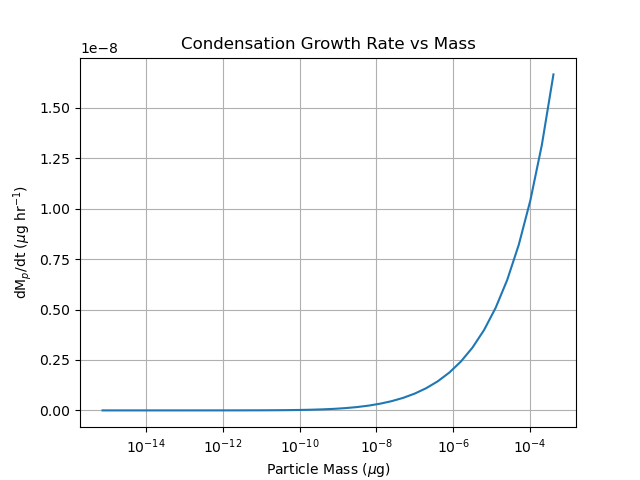
\includegraphics[width=5in]{hw2_pr1_2_condensation_growth_rate_vs_mass.png}
        \caption{Problem(1) part(b) Condensation mass growth rate vs particle diameter}
    \end{center}
\end{figure}




%new page
\newpage
\section{GDE Coagulation}\label{sec:problem-2}
% part A of problem 2 % subsection written in form of 2.a
\begin{figure}\label{fig:problem-2-a-1}
\begin{center}
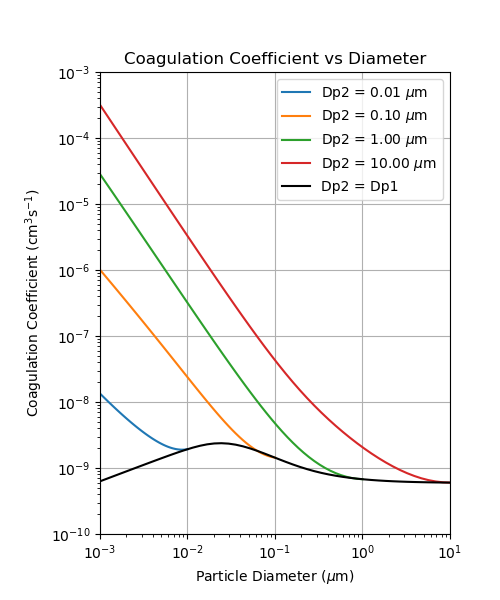
\includegraphics[width=3in]{hw2_pr2_1_coagulation_coefficient_vs_diameter}
\caption{Fuchs Coagulation the code}
\end{center}
\end{figure}

\newpage
\section{Condensation + Coagulation}\label{sec:problem-2}

\begin{figure}\label{fig:problem-2-a-1}
\begin{center}
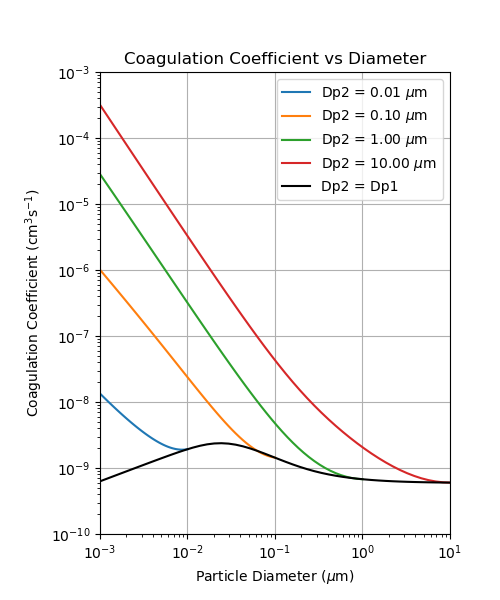
\includegraphics[width=3in]{hw2_pr2_1_coagulation_coefficient_vs_diameter}
\caption{Fuchs Coagulation the code}
\end{center}
\end{figure}

\begin{figure}\label{fig:problem-2-a-2}
\begin{center}
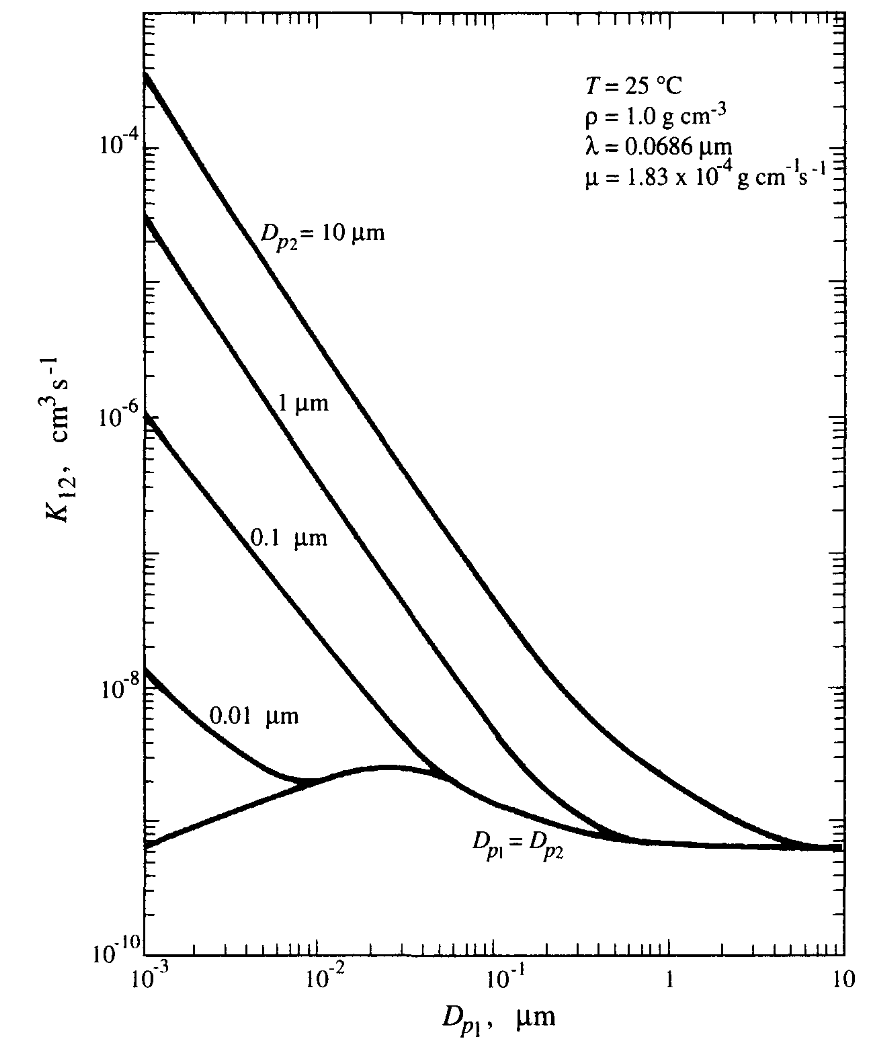
\includegraphics[width=3in]{Table_13_5_Fuchs_Coagulation_plot.png}
\caption{Table\_13\_5 Fuchs Coagulation plot}
\end{center}
\end{figure}



\end{document}


